\documentclass[12pt,a4paper]{article}

% ─── Page Layout ───────────────────────────────────────────────────────────────
\usepackage[a4paper, margin=0.8in, headheight=14pt]{geometry}

% ─── Fonts (XeLaTeX) ───────────────────────────────────────────────────────────
\usepackage{fontspec}
\usepackage{unicode-math}
\setmainfont{TeX Gyre Pagella}
\setmonofont[Scale=0.88]{TeX Gyre Cursor}
\setmathfont{Latin Modern Math}

% ─── Packages ──────────────────────────────────────────────────────────────────
\usepackage{xcolor}
\usepackage{colortbl}
\usepackage{titlesec}
\usepackage{enumitem}
\usepackage{tabularx}
\usepackage{booktabs}
\usepackage{array}
\usepackage{amsmath}
\usepackage{tikz}
\usetikzlibrary{shapes.geometric, arrows.meta, positioning, calc, fit, decorations.pathreplacing}
\usepackage{tcolorbox}
\tcbuselibrary{skins, breakable}
\usepackage{hyperref}
\usepackage{fancyhdr}
\usepackage{graphicx}
\usepackage{microtype}
\hyphenpenalty=10000
\exhyphenpenalty=10000
\sloppy
\usepackage{caption}
\usepackage{setspace}
\usepackage{multirow}
\usepackage{tocloft}

% ─── Q&A helper ────────────────────────────────────────────────────────────────
\newcommand{\Q}[1]{\textbf{#1}\par\noindent\ignorespaces}

% ─── Colour Palette ────────────────────────────────────────────────────────────
\definecolor{myred}{RGB}{196,30,58}
\definecolor{mydark}{RGB}{30,30,50}
\definecolor{mygreen}{RGB}{14,120,80}
\definecolor{myteal}{RGB}{0,130,140}
\definecolor{myamber}{RGB}{180,100,0}
\definecolor{mypurple}{RGB}{100,30,160}
\definecolor{mygray}{RGB}{246,247,249}
\definecolor{mgframe}{RGB}{180,185,200}
\definecolor{watermark}{RGB}{145,150,170}
\definecolor{hdrred}{RGB}{250,232,235}
\definecolor{hdrgreen}{RGB}{220,244,233}
\definecolor{hdrteal}{RGB}{220,242,244}
\definecolor{hdramber}{RGB}{253,242,215}
\definecolor{hdrpurple}{RGB}{238,228,255}
\definecolor{hdrgray}{RGB}{238,240,245}
\definecolor{rowalt}{RGB}{250,251,253}

% ─── Section Formatting ────────────────────────────────────────────────────────
\titleformat{\section}
  {\large\bfseries\color{myred}}{\thesection.}{0.5em}{}
  [\vspace{1pt}{\color{myred}\rule{\linewidth}{0.8pt}}]
\titleformat{\subsection}
  {\normalsize\bfseries\color{myteal}}{\thesubsection}{0.5em}{}
\titlespacing*{\section}{0pt}{18pt}{7pt}
\titlespacing*{\subsection}{0pt}{11pt}{4pt}

% ─── Paragraph ─────────────────────────────────────────────────────────────────
\setlength{\parindent}{0pt}
\setlength{\parskip}{4pt}

% ─── TOC Styling ───────────────────────────────────────────────────────────────
\renewcommand{\cfttoctitlefont}{\large\bfseries\color{myred}}
\renewcommand{\cftaftertoctitle}{\par\noindent{\color{myred}\rule{\linewidth}{0.8pt}}}
\setlength{\cftbeforetoctitleskip}{0pt}
\setlength{\cftaftertoctitleskip}{6pt}
\renewcommand{\cftsecfont}{\normalsize\bfseries\color{mydark}}
\renewcommand{\cftsecpagefont}{\normalsize\bfseries\color{mydark}}
\renewcommand{\cftsecleader}{\cftdotfill{\cftdotsep}}
\setlength{\cftbeforesecskip}{7pt}
\renewcommand{\cftsubsecfont}{\small\color{mydark}}
\renewcommand{\cftsubsecpagefont}{\small\color{mydark}}
\setlength{\cftbeforesubsecskip}{3pt}
\setlength{\cftsubsecindent}{1.4em}

% ─── Table helpers ─────────────────────────────────────────────────────────────
\renewcommand{\arraystretch}{1.45}
\setlength{\tabcolsep}{6pt}
\arrayrulecolor{mydark}
\newcolumntype{B}[1]{>{\small\bfseries\raggedright\arraybackslash}m{#1}}
\newcolumntype{Y}{>{\small\raggedright\arraybackslash}X}
\renewcommand{\tabularxcolumn}[1]{m{#1}}

% ─── Header / Footer ───────────────────────────────────────────────────────────
\pagestyle{fancy}
\fancyhf{}
\fancyhead[L]{\small\color{myred}\textbf{PE-EC801A}\;\color{mydark}--- Antennas and Propagation}
\fancyhead[R]{\small\color{myteal}\textbf{Module 5 Notes}}
\fancyfoot[C]{\small\color{mydark}\thepage}
\fancyfoot[R]{\small\color{watermark}\textit{\copyright\ Biraj}}
\renewcommand{\headrulewidth}{0.5pt}
\renewcommand{\footrulewidth}{0.3pt}

% ─── Hyperref ──────────────────────────────────────────────────────────────────
\hypersetup{
  colorlinks=true, linkcolor=myteal, urlcolor=myteal,
  pdfauthor={Biraj Sarkar},
  pdftitle={PE-EC801A --- Module 5 Notes}
}

% ─── tcolorbox styles ──────────────────────────────────────────────────────────
\tcbset{
  tikzbox/.style={
    colback=mygray, colframe=mgframe, boxrule=0.6pt, arc=4pt,
    left=8pt, right=8pt, top=6pt, bottom=6pt,
    colbacktitle=mgframe, coltitle=mydark,
    fonttitle=\small\bfseries
  },
  defbox/.style={
    colback=hdrgreen, colframe=mygreen, boxrule=0.8pt, arc=4pt,
    left=9pt, right=9pt, top=6pt, bottom=6pt,
    colbacktitle=mygreen, coltitle=white,
    fonttitle=\small\bfseries
  },
  formulabox/.style={
    colback=hdrteal, colframe=myteal, boxrule=0.8pt, arc=4pt,
    left=9pt, right=9pt, top=7pt, bottom=7pt,
    colbacktitle=myteal, coltitle=white,
    fonttitle=\small\bfseries
  },
  examplebox/.style={
    colback=hdramber, colframe=myamber, boxrule=0.8pt, arc=4pt,
    left=9pt, right=9pt, top=6pt, bottom=6pt,
    colbacktitle=myamber, coltitle=white,
    fonttitle=\small\bfseries
  },
  masonbox/.style={
    colback=hdrpurple, colframe=mypurple, boxrule=0.8pt, arc=4pt,
    left=9pt, right=9pt, top=6pt, bottom=6pt,
    colbacktitle=mypurple, coltitle=white,
    fonttitle=\small\bfseries
  },
  exambox/.style={
    colback=hdrpurple, colframe=mypurple, boxrule=1pt, arc=5pt,
    left=10pt, right=10pt, top=8pt, bottom=8pt,
    colbacktitle=mypurple, coltitle=white,
    fonttitle=\bfseries,
    breakable, title after break={\textbf{Frequently Asked / Viva Questions (contd.)}}}
}
\tcbset{breakable}

% ─── TikZ styles ───────────────────────────────────────────────────────────────
\tikzset{
  block/.style={rectangle, draw=myteal, fill=hdrteal,
    text width=2.4cm, align=center, minimum height=0.95cm,
    font=\small, rounded corners=3pt, line width=0.7pt},
  redblock/.style={rectangle, draw=myred, fill=hdrred,
    text width=2.4cm, align=center, minimum height=0.95cm,
    font=\small, rounded corners=3pt, line width=0.7pt},
  netnode/.style={rectangle, draw=myteal, fill=hdrteal,
    text width=1.5cm, align=center, minimum height=0.8cm,
    font=\small, rounded corners=3pt, line width=0.7pt},
  sumjunc/.style={circle, draw=myamber, fill=hdramber,
    minimum size=0.62cm, font=\small, line width=0.8pt},
  snode/.style={circle, draw=mypurple, fill=hdrpurple,
    minimum size=0.55cm, font=\footnotesize, line width=0.7pt},
  arrow/.style={-Stealth, thick, color=mydark},
  redarrow/.style={-Stealth, thick, color=myred},
  line/.style={thick, color=mydark}
}

% ═══════════════════════════════════════════════════════════════════════════════
\begin{document}
% ═══════════════════════════════════════════════════════════════════════════════

\begin{center}
  {\LARGE\bfseries\color{myred} PE-EC801A --- Antennas and Propagation}\\[5pt]
  {\normalsize\color{mydark} Semester VIII \quad$\bullet$\quad 3L:0T:0P \quad$\bullet$\quad 3 Credits}\\[3pt]
  {\normalsize\color{myteal}\textbf{Module 5 Exam Notes}}\\[3pt]
  {\small\color{mydark} CGEC \;$|$\; B.Tech ECE (2023--27) \;$|$\; \textit{Biraj Sarkar}}
\end{center}
\vspace{2pt}
\noindent{\color{myred}\rule{\linewidth}{1.5pt}}
\vspace{2pt}

\hypersetup{linkcolor=mydark}
\tableofcontents
\hypersetup{linkcolor=myteal}
\newpage

% ===============================================================================
\section{Characteristics of Microstrip Antennas}
% ===============================================================================

\begin{tcolorbox}[defbox, title={\textbf{Definition of Microstrip Patch Antenna}}]
A \textbf{microstrip patch antenna} consists of a radiating metallic patch (usually rectangular or circular) etched on one side of a thin, grounded dielectric substrate (dielectric constant $\epsilon_r$ and thickness $h$, where $h \ll \lambda$).
\end{tcolorbox}

\subsection{Physical Structure and Radiation Mechanism}
The metallic patch is usually made of copper or gold. The substrate thickness is typically $0.003\lambda_0 \le h \le 0.05\lambda_0$.
The patch acts as a resonant cavity with open-circuited edges. Fringing fields at the edges of the patch (along the length) act as the source of radiation. These fields extend slightly outside the physical boundaries, meaning the patch behaves electrically as if it were slightly larger than its physical dimensions.

\begin{tcolorbox}[tikzbox, title={Rectangular Microstrip Patch Antenna (Cross-Section and Top View)}]
\centering
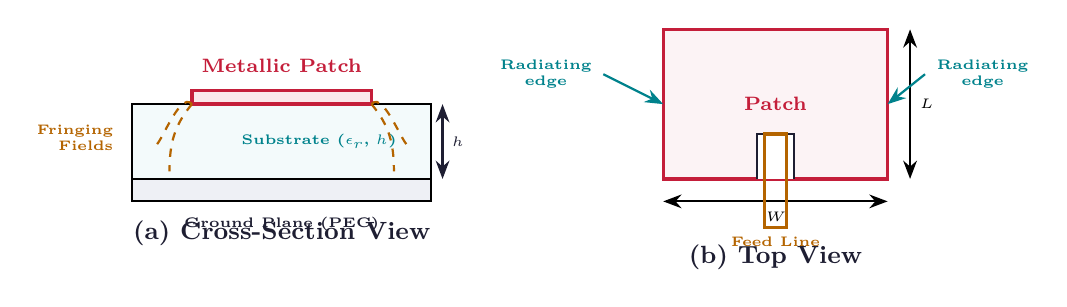
\begin{tikzpicture}[scale=0.95]
  % ── Cross-section view (left) ──────────────────────────────────────────────
  \begin{scope}[xshift=-3.8cm]
    % Ground plane
    \draw[thick, fill=hdrgray] (-2.0,-1.3) rectangle (2.0,-1.0);
    \node[below=2pt, font=\tiny\bfseries\color{mydark}] at (0,-1.3) {Ground Plane (PEC)};
    % Substrate
    \draw[thick, fill=hdrteal, fill opacity=0.35] (-2.0,-1.0) rectangle (2.0,0.0);
    \node[font=\tiny\bfseries\color{myteal}] at (0.5,-0.5) {Substrate ($\epsilon_r$, $h$)};
    % Patch
    \draw[very thick, color=myred, fill=hdrred] (-1.2,0.0) rectangle (1.2,0.18);
    \node[above=3pt, font=\scriptsize\bfseries\color{myred}] at (0,0.18) {Metallic Patch};
    % Fringing fields at left edge
    \draw[thick, color=myamber, dashed] (-1.2, 0.0) to[out=130, in=270] (-1.7, -0.5);
    \draw[thick, color=myamber, dashed] (-1.2, 0.0) to[out=230, in=90] (-1.5, -0.9);
    % Fringing fields at right edge
    \draw[thick, color=myamber, dashed] (1.2, 0.0) to[out=50, in=270] (1.7, -0.5);
    \draw[thick, color=myamber, dashed] (1.2, 0.0) to[out=-50, in=90] (1.5, -0.9);
    % Fringing label on left, clear of substrate text
    \node[left=2pt, align=right, font=\tiny\bfseries\color{myamber}] at (-2.05, -0.45) {Fringing\\Fields};
    % Height annotation
    \draw[Stealth-Stealth, thick, color=mydark] (2.15,-1.0) -- (2.15, 0.0) node[midway, right, font=\tiny] {$h$};
    \node[font=\small\bfseries\color{mydark}] at (0,-1.72) {(a) Cross-Section View};
  \end{scope}

  % ── Top view (right) ───────────────────────────────────────────────────────
  \begin{scope}[xshift=2.8cm]
    % Patch boundary
    \draw[very thick, color=myred, fill=hdrred, fill opacity=0.5] (-1.5,-1.0) rectangle (1.5,1.0);
    \node[font=\scriptsize\bfseries\color{myred}] at (0,0) {Patch};
    % W dimension
    \draw[Stealth-Stealth, thick] (-1.5,-1.3) -- (1.5,-1.3) node[midway, below, font=\tiny] {$W$};
    % L dimension
    \draw[Stealth-Stealth, thick] (1.8,-1.0) -- (1.8,1.0) node[midway, right, font=\tiny] {$L$};
    % Inset feed notch
    \fill[white] (-0.25,-1.0) rectangle (0.25,-0.4);
    \draw[thick, color=mydark] (-0.25,-1.0) -- (-0.25,-0.4) -- (0.25,-0.4) -- (0.25,-1.0);
    % Feed line
    \draw[very thick, color=myamber] (-0.15,-1.65) rectangle (0.15,-0.4);
    \node[below, font=\tiny\bfseries\color{myamber}] at (0,-1.65) {Feed Line};
    % Radiating edges label
    \draw[Stealth-, thick, color=myteal] (-1.5, 0.0) -- (-2.3, 0.4) node[left, align=center, text width=1.2cm, font=\tiny\bfseries\color{myteal}] {Radiating edge};
    \draw[Stealth-, thick, color=myteal] (1.5, 0.0) -- (2.0, 0.4) node[right, align=center, text width=1.2cm, font=\tiny\bfseries\color{myteal}] {Radiating edge};
    \node[font=\small\bfseries\color{mydark}] at (0,-2.05) {(b) Top View};
  \end{scope}
\end{tikzpicture}
\end{tcolorbox}

\par\noindent
\textbf{Advantages and Disadvantages:}\par\noindent
{\renewcommand{\arraystretch}{1.45}%
\begin{tabularx}{\linewidth}{|Y|Y|}
\hline
\textbf{Advantages} & \textbf{Disadvantages} \\
\hline
Low profile, lightweight, conformable to surfaces. & Extremely narrow bandwidth (typically $1\%$–$5\%$). \\
\hline
Low fabrication cost (easy to print on PCBs). & Low radiation efficiency (due to dielectric and surface losses). \\
\hline
Supports dual-frequency and dual-polarization. & Low power handling capability. \\
\hline
\end{tabularx}}

% ===============================================================================
\section{Feeding Methods}
% ===============================================================================

To transfer electromagnetic energy into the patch, several feed techniques are used:

\begin{enumerate}[label=\textbf{\arabic*.}, leftmargin=*, itemsep=4pt]
  \item \textbf{Microstrip Line Feed:} A microstrip conducting strip feed is directly connected to the edge of the patch.
    \begin{itemize}[leftmargin=*, itemsep=1pt]
      \item \textit{Match method:} Inset cuts are made in the patch to match the high patch edge impedance to the feed line.
      \item \textit{Pros/Cons:} Easy to fabricate; but causes spurious feed radiation.
    \end{itemize}
  \item \textbf{Coaxial Probe Feed:} The outer conductor of a coaxial cable is connected to the ground plane, and the inner pin extends through the substrate and is soldered to the patch.
    \begin{itemize}[leftmargin=*, itemsep=1pt]
      \item \textit{Match method:} Match is achieved by choosing the insertion point offset from the patch edges.
      \item \textit{Pros/Cons:} Low spurious radiation; but requires drilling holes, making it harder to fabricate.
    \end{itemize}
  \item \textbf{Aperture-Coupled Feed:} The feed line is on a lower substrate, separated from the patch substrate by a common ground plane. Coupling occurs via a slot/aperture cut in the ground plane.
    \begin{itemize}[leftmargin=*, itemsep=1pt]
      \item \textit{Pros/Cons:} Shields feed line spurious radiation, improves bandwidth; but requires multilayer fabrication.
    \end{itemize}
  \item \textbf{Proximity-Coupled Feed:} The feed line is sandwiched between two substrate layers, and the patch is on the top surface. Energy couples electromagnetically.
    \begin{itemize}[leftmargin=*, itemsep=1pt]
      \item \textit{Pros/Cons:} Widest bandwidth (up to $13\%$), no contact needed; but complex to align.
    \end{itemize}
\end{enumerate}

\begin{tcolorbox}[tikzbox, title={Microstrip Line Feed vs. Coaxial Probe Feed}]
\centering
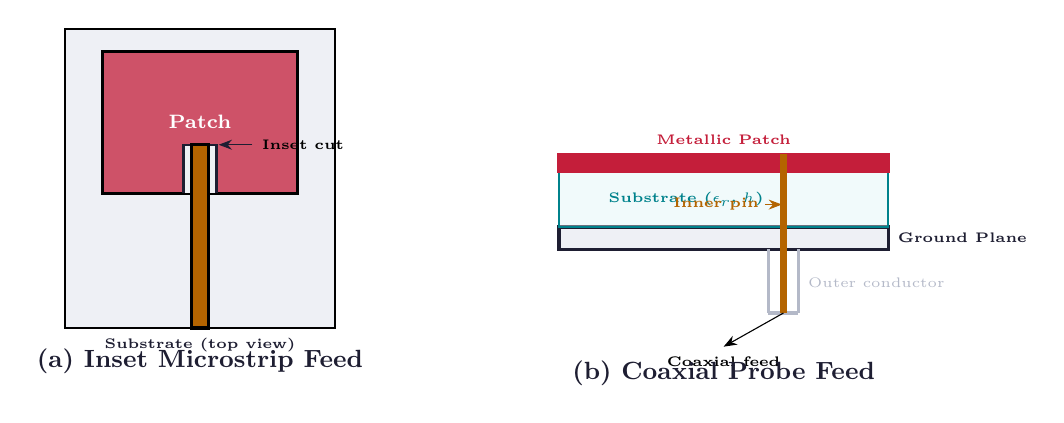
\begin{tikzpicture}[scale=0.95]
  % ── (a) Inset Microstrip Line Feed (top view) ──────────────────────────────
  \begin{scope}[xshift=-3.8cm]
    % Substrate / ground boundary shown as outer box
    \draw[thick, fill=hdrgray] (-1.8,-2.1) rectangle (1.8,1.9);
    \node[below, font=\tiny\bfseries\color{mydark}] at (0,-2.1) {Substrate (top view)};
    % Patch
    \draw[very thick, fill=myred, fill opacity=0.75] (-1.3,-0.3) rectangle (1.3,1.6);
    \node[font=\scriptsize\bfseries\color{white}] at (0, 0.65) {Patch};
    % Inset notch cut into patch
    \fill[hdrgray] (-0.22,-0.3) rectangle (0.22,0.35);
    \draw[thick, color=mydark] (-0.22,-0.3) -- (-0.22,0.35) -- (0.22,0.35) -- (0.22,-0.3);
    % Feed line (amber strip coming from bottom)
    \draw[very thick, fill=myamber] (-0.11,-2.1) rectangle (0.11,0.35);
    % Inset feed label
    \draw[-Stealth, thin, color=mydark] (0.7, 0.35) -- (0.25, 0.35);
    \node[right, font=\tiny\bfseries] at (0.7, 0.35) {Inset cut};
    % Dimension arrows
    \node[font=\tiny\bfseries\color{myamber}, below] at (0,-2.1) {};
    \node[font=\small\bfseries\color{mydark}] at (0,-2.55) {(a) Inset Microstrip Feed};
  \end{scope}

  % ── (b) Coaxial Probe Feed (cross-section view) ────────────────────────────
  \begin{scope}[xshift=3.2cm]
    % Ground plane (thick copper bar)
    \draw[very thick, fill=hdrgray, draw=mydark] (-2.2,-1.05) rectangle (2.2,-0.75);
    \node[right, font=\tiny\bfseries\color{mydark}] at (2.2,-0.9) {Ground Plane};
    % Substrate layer
    \draw[thick, fill=hdrteal, fill opacity=0.4, draw=myteal]
      (-2.2,-0.75) rectangle (2.2,0.0);
    \node[font=\tiny\bfseries\color{myteal}] at (-0.5,-0.38) {Substrate ($\epsilon_r$, $h$)};
    % Patch (top copper strip)
    \draw[very thick, fill=myred, draw=myred] (-2.2,0.0) rectangle (2.2,0.22);
    \node[above, font=\tiny\bfseries\color{myred}] at (0,0.22) {Metallic Patch};
    % Outer conductor of coax (below ground)
    \draw[very thick, color=mgframe] (0.6,-1.05) -- (0.6,-1.9);
    \draw[very thick, color=mgframe] (1.0,-1.05) -- (1.0,-1.9);
    \draw[very thick, color=mgframe] (0.6,-1.9) -- (1.0,-1.9);
    \node[right, font=\tiny\color{mgframe}] at (1.0,-1.5) {Outer conductor};
    % Inner pin (amber, goes through substrate to patch)
    \draw[line width=2.5pt, color=myamber] (0.8,-1.9) -- (0.8, 0.22);
    \node[left, font=\tiny\bfseries\color{myamber}] at (0.6,-0.45) {Inner pin};
    \draw[-Stealth, thin, color=myamber] (0.55,-0.45) -- (0.78,-0.45);
    % Coax label at bottom
    \draw[-Stealth, thin] (0.8,-1.9) -- (0.0,-2.35) node[below, font=\tiny\bfseries] {Coaxial feed};
    \node[font=\small\bfseries\color{mydark}] at (0,-2.7) {(b) Coaxial Probe Feed};
  \end{scope}
\end{tikzpicture}
\end{tcolorbox}

% ===============================================================================
\section{Methods of Analysis}
% ===============================================================================

\begin{itemize}[leftmargin=*, itemsep=3pt]
  \item \textbf{Transmission Line Model:} Simplest model. It represents the patch as a microstrip transmission line of length $L$ terminated by two radiating slots (modeled as parallel conductances $G$ and susceptances $B$). It yields good physical insight but is less accurate.
  \item \textbf{Cavity Model:} Represents the region between the patch and ground plane as a dielectric-loaded cavity with electric conductors on top/bottom, and artificial magnetic walls along the patch edges. It is more accurate and models higher-order modes.
  \item \textbf{Full-Wave Models:} Numerical techniques (such as the Method of Moments (MoM), Finite Element Method (FEM), or Finite Difference Time Domain (FDTD)). They are highly accurate for arbitrary shapes but are computationally demanding.
\end{itemize}

% ===============================================================================
\section{Design of Rectangular and Circular Patch Antennas}
% ===============================================================================

\subsection{Rectangular Patch Antenna Design}
The design parameters are: substrate height $h$, dielectric constant $\epsilon_r$, and resonant frequency $f_r$.

\begin{tcolorbox}[formulabox, title={\textbf{Rectangular Patch Design Calculations}}]
\begin{enumerate}[leftmargin=*, label=\textbf{\arabic*.}, itemsep=3pt, topsep=1pt]
  \item \textbf{Width ($W$):} To ensure high radiation efficiency, the width is:
  \[
  W = \frac{v_0}{2 f_r} \sqrt{\frac{2}{\epsilon_r + 1}}
  \]
  where $v_0 \approx 3 \times 10^8\,\text{m/s}$.
  \item \textbf{Effective Dielectric Constant ($\epsilon_{reff}$):} Accounts for fringing fields:
  \[
  \epsilon_{reff} = \frac{\epsilon_r + 1}{2} + \frac{\epsilon_r - 1}{2} \left[ 1 + 12 \frac{h}{W} \right]^{\!-1/2}
  \]
  \item \textbf{Extended Patch Length ($\Delta L$):} Due to fringing fields:
  \[
  \Delta L = 0.412 h \frac{(\epsilon_{reff} + 0.3)\left(\frac{W}{h} + 0.264\right)}{(\epsilon_{reff} - 0.258)\left(\frac{W}{h} + 0.8\right)}
  \]
  \item \textbf{Physical Length ($L$):}
  \[
  L = L_{eff} - 2\Delta L = \frac{v_0}{2 f_r \sqrt{\epsilon_{reff}}} - 2\Delta L
  \]
\end{enumerate}
\end{tcolorbox}

\subsection{Circular Patch Antenna Design}
For a circular patch of radius $a$ on a substrate of height $h$, the dominant resonant mode is $TM^z_{110}$.

\begin{tcolorbox}[formulabox, title={\textbf{Circular Patch Design Equations}}]
The physical radius $a$ is calculated as:
\[
a = \frac{F}{\left\{ 1 + \frac{2h}{\pi \epsilon_r F} \left[ \ln\left(\frac{\pi F}{2h}\right) + 1.7726 \right] \right\}^{1/2}}
\]
where:
\[
F = \frac{8.791 \times 10^9}{f_r \sqrt{\epsilon_r}} \quad (\text{for } f_r \text{ in Hz})
\]
The effective radius $a_e$ incorporating fringing fields is:
\[
a_e = a \left\{ 1 + \frac{2h}{\pi \epsilon_r a} \left[ \ln\left(\frac{\pi a}{2h}\right) + 1.7726 \right] \right\}^{1/2}
\]
The resonant frequency for the $TM^z_{110}$ mode is:
\[
(f_r)_{110} = \frac{1.8412 v_0}{2\pi a_e \sqrt{\epsilon_r}}
\]
\end{tcolorbox}

% ===============================================================================
% MANDATORY QUICK REVISION PAGE
% ===============================================================================
\newpage
\begin{center}
  {\large\bfseries\color{myred} Quick Revision --- Module 5}\\[3pt]
  {\small\color{mydark} Microstrip Antennas $|$ PE-EC801A}
\end{center}
\noindent{\color{myred}\rule{\linewidth}{1.2pt}}
\vspace{4pt}

\begin{tcolorbox}[formulabox, title={\textbf{Key Formulas and Metrics at a Glance}}]
\renewcommand{\arraystretch}{1.35}
\begin{tabularx}{\linewidth}{B{5.2cm} X}
Rectangular Patch Width ($W$) & $W = \frac{v_0}{2 f_r} \sqrt{\frac{2}{\epsilon_r + 1}}$ \\[4pt]
Effective Dielectric ($\epsilon_{reff}$) & $\epsilon_{reff} = \frac{\epsilon_r + 1}{2} + \frac{\epsilon_r - 1}{2} \left[ 1 + 12 \frac{h}{W} \right]^{-1/2}$ \\[4pt]
Extended Length ($\Delta L$) & $\Delta L \approx 0.412 h \frac{(\epsilon_{reff} + 0.3)(W/h + 0.264)}{(\epsilon_{reff} - 0.258)(W/h + 0.8)}$ \\[4pt]
Physical Length ($L$) & $L = \frac{v_0}{2 f_r \sqrt{\epsilon_{reff}}} - 2\Delta L$ \\[4pt]
Resonant circular frequency & $(f_r)_{110} = \frac{1.8412 v_0}{2\pi a_e \sqrt{\epsilon_r}}$ \\[4pt]
Effective circular radius ($a_e$) & $a_e = a \left\{ 1 + \frac{2h}{\pi \epsilon_r a} \left[ \ln\left(\frac{\pi a}{2h}\right) + 1.7726 \right] \right\}^{1/2}$ \\
\end{tabularx}
\end{tcolorbox}

\begin{tcolorbox}[defbox, title={\textbf{One-Line Definitions}}]
\begin{itemize}[leftmargin=*, itemsep=2pt, topsep=0pt]
  \item \textbf{Fringing Fields:} The bending of electric field lines at the open-circuit boundaries of a microstrip patch, which enables radiation.
  \item \textbf{Inset Feed:} A feed technique where notch cuts are made in the patch to match the low line impedance ($\approx 50\,\Omega$) directly inside the patch.
  \item \textbf{Transmission Line Model:} An analytical model that treats a rectangular patch antenna as two radiating slots separated by a transmission line.
  \item \textbf{Cavity Model:} An analysis model that treats the patch as a cavity bounded by perfect electric and magnetic walls.
  \item \textbf{Full-Wave Analysis:} Direct numerical solvers of Maxwell's equations (e.g., FEM, FDTD) used for complex microstrip geometries.
\end{itemize}
\end{tcolorbox}

\begin{tcolorbox}[exambox, title={\textbf{Frequently Asked / Viva Questions}}]
\begin{enumerate}[topsep=0pt, label=\textbf{Q\arabic*.}, itemsep=5pt]
  \item \Q{What is the primary mechanism of radiation in microstrip patch antennas?}
    Radiation is generated by the fringing fields at the patch edges. These fringing fields act as slot sources along the radiating edges (separated by $L \approx \lambda/2$).
  \item \Q{Compare microstrip line feeding and coaxial probe feeding.}
    Microstrip line feeds are simple to fabricate but introduce spurious radiation from the feed line, which degrades the radiation pattern. Coaxial probe feeding offers lower spurious radiation and easy matching, but requires drilling holes, making fabrication more complex.
  \item \Q{What is the purpose of an inset feed in microstrip antennas?}
    The input impedance at the edge of a patch is high (typically $200$–$300\,\Omega$). An inset notch shifts the contact point of the feed line toward the center of the patch, where the impedance is lower, matching it to a standard $50\,\Omega$ transmission line.
  \item \Q{Why does a microstrip patch antenna have a narrow bandwidth?}
    The patch antenna behaves electrically as a high-Q resonant cavity with a small volume. Since the substrate height $h$ is thin ($h \ll \lambda$), the energy stored in the cavity is high compared to the energy radiated, leading to a narrow bandwidth.
  \item \Q{Explain the physical meaning of the effective dielectric constant ($\epsilon_{reff}$).}
    Because the fringing field lines travel partly through the dielectric substrate and partly through the surrounding air, the wave behaves as if it were propagating through a homogeneous medium with a dielectric constant $\epsilon_{reff}$ that lies between $1$ (air) and $\epsilon_r$ (substrate).
  \item \Q{State the advantages of aperture-coupled feeds over direct feeding methods.}
    The ground plane separates the feed line from the radiating patch, preventing spurious feed line radiation from distorting the antenna's far-field radiation pattern. It also allows independent optimization of the feed and patch substrate thicknesses.
\end{enumerate}
\end{tcolorbox}

\begin{tcolorbox}[tikzbox, title={Comparison of Patch Feeding Methods}]
\centering
\renewcommand{\arraystretch}{1.55}
{\renewcommand{\arraystretch}{1.55}%
\begin{tabularx}{\linewidth}{|B{3.2cm}|Y|Y|Y|}
\hline
\multicolumn{1}{|>{\centering\arraybackslash}m{3.2cm}|}{\textbf{Feed Type}} &
\multicolumn{1}{>{\centering\arraybackslash}Y|}{\textbf{Ease of Fab}} &
\textbf{Spurious Radiation} &
\textbf{Relative Bandwidth} \\
\hline
Microstrip Line & Very Easy & High & Narrow ($1$–$2\%$) \\
\hline
Coaxial Probe & Moderate (requires drilling) & Low & Narrow ($1$–$3\%$) \\
\hline
Aperture Coupled & Complex (multilayer alignment) & Lowest (shielded by ground) & Moderate ($4$–$5\%$) \\
\hline
Proximity Coupled & Complex (multilayer alignment) & Low & Widest ($10$–$13\%$) \\
\hline
\end{tabularx}}
\end{tcolorbox}

\end{document}
